% !TEX TS-program = pdflatex
% !TEX encoding = UTF-8 Unicode

% This is a simple template for a LaTeX document using the "article" class.
% See "book", "report", "letter" for other types of document.

\documentclass[11pt]{article} % use larger type; default would be 10pt

\usepackage[utf8]{inputenc} % set input encoding (not needed with XeLaTeX)

%%% Examples of Article customizations
% These packages are optional, depending whether you want the features they provide.
% See the LaTeX Companion or other references for full information.

%%% PAGE DIMENSIONS
\usepackage{geometry} % to change the page dimensions
\geometry{a4paper} % or letterpaper (US) or a5paper or....
\geometry{margin=1in} % for example, change the margins to 2 inches all round
% \geometry{landscape} % set up the page for landscape
%   read geometry.pdf for detailed page layout information

\usepackage{graphicx} % support the \includegraphics command and options

\usepackage[parfill]{parskip} % Activate to begin paragraphs with an empty line rather than an indent
\setlength{\parindent}{1cm}

%%% PACKAGES
\usepackage{booktabs} % for much better looking tables
\usepackage{array} % for better arrays (eg matrices) in maths
\usepackage{paralist} % very flexible & customisable itemizes (eg. enumerate/itemize, etc.)
\usepackage{verbatim} % adds environment for commenting out blocks of text & for better verbatim
\usepackage{subfig} % make it possible to include more than one captioned figure/table in a single float
\usepackage{amssymb} % more 'unusual' symbols not included in standard LaTeX package
\usepackage{enumitem}
\usepackage{amsmath}
\usepackage{comment}
\usepackage{multirow}
\usepackage{color}
\usepackage{graphicx}
\usepackage{xspace}
\usepackage{gensymb}
\usepackage[font=footnotesize,format=plain,labelfont=bf,textfont=bf ,justification=justified,singlelinecheck=false]{caption}
\usepackage{calligra}
\DeclareMathAlphabet{\mathcalligra}{T1}{calligra}{m}{n} 
\DeclareFontShape{T1}{calligra}{m}{n}{<->s*[2.2]callig15}{} 
\usepackage{dcolumn}
\newcolumntype{d}[1]{D{.}{\cdot}{#1} }
\newcommand{\centercell}[1]{\multicolumn{1}{C}{#1}}

% These packages are all incorporated in the memoir class to one degree or another...

%%% HEADERS & FOOTERS
\usepackage{fancyhdr} % This should be set AFTER setting up the page geometry
\pagestyle{fancy} % options: empty , plain , fancy
\renewcommand{\headrulewidth}{0pt} % customise the layout...
\lhead{}\chead{}\rhead{}
\lfoot{}\cfoot{\thepage}\rfoot{}


%%% SECTION TITLE APPEARANCE
\usepackage{sectsty}
\allsectionsfont{\sffamily\mdseries\upshape} % (See the fntguide.pdf for font help)
% (This matches ConTeXt defaults)

%%% ToC (table of contents) APPEARANCE
\usepackage[nottoc,notlof,notlot]{tocbibind} % Put the bibliography in the ToC
\usepackage[titles,subfigure]{tocloft} % Alter the style of the Table of Contents
\renewcommand{\cftsecfont}{\rmfamily\mdseries\upshape}
\renewcommand{\cftsecpagefont}{\rmfamily\mdseries\upshape} % No bold!

%%%Command Macros


%%% END Article customizations

\graphicspath{ {./images/} }

\title{The Mimas Leading Edge Anomaly: Thermal conductivity and grain cementation radius}
\author{M.J. Schaible, R.Johnson, L. Zhigilei}
%\date{} % Activate to display a given date or no date (if empty),
         % otherwise the current date is printed 

\begin{document}
\maketitle

\section{Goals}

	\begin{itemize}
	\item Derive the thermal conductivity differences between inside/outside anomalous region on Mimas and Tethys
		\begin{itemize}
		\item Can the thermal conductivity differences be explained in terms of structural differences in the regolith?
		\item How does the thermal conductivity depend on grain contact: linearly or quadratically?
		\item Is Hertzian analysis sufficient to determine effective contact areas between grains?
		\end{itemize}
	\item Estimate effects of $>$1MeV electrons on grain cementation properties
		\begin{itemize}
		\item Determine energy deposition vs. depth profile of the electrons in the regolith from PENELOPE results.
		\item What is the heating effect on $\sim$50$\mu$m grains for each interaction?
		\item What are the relative thermal and near surface electronic excitation molecular desorption yields from pore surfaces?
			\begin{itemize}
			\item Use energy vs. depth to estimate grain heating for input into sintering equations. 
			\item Use thermal spike method to model electronic excitation desorption.
			\item How can Hayley simulations be used to help understand?
			\end{itemize}
		\item What is the gas production rate? How do gas readsorption time-scales compare to heat transfer time-scales?
		\item What are electron effects on crystal structure, esp. at the grain boundary? (comment)
		\item Using energy deposition profile and known W-value, estimate probability of excitations.
		\item Can the electron irradiation explain thermal conductivity differences?
		\end{itemize}
%	\item Estimate the proton defect creation, sintering, and gas production rates. Can they account for trailing hemisphere discolorations?
	\item Estimate time-scale for cementation increase to explain increased cementation
	\item Use published results to estimate gardening rate due to micrometeorite bombardment and compare to sintering time-scale.
	\end{itemize}

	Thermal models have been developed to simulate heat transport in planetary and cometary surfaces. These models depend on the thermal conductivity of the bulk material making up the grains in the regolith, the porosity ($\phi$) and on geometric factors that describe the packing of grains. For the case of an icy regolith on an airless body in the outer solar system, contributions to thermal conductivity other than conduction through grains (i.e. radiative, convective, latent heat) can be shown to be negligible.

\section{Introduction}
\label{sec:intro}

	Analysis of Cassini photometry data revealed an anomalous region present on the leading edge of the Saturnian icy moons Mimas and Tethys. The feature extends over the entire width of the leading hemisphere and $\sim\pm40\degree$ and $\sim\pm20\degree$ to the north and south at the center of the lens for Mimas and Tethys respectively, though it narrows to within a few degrees at the edges of the hemisphere for both moons. The feature is dark in IR (0.930 $\mu$m) and Green (0.568 $mu$m) bands but bright in the UV (0.338 $\mu$m) as shown by albedo maps [Elderetal2007; Shenketal2011]. The smaller IR/UV ratio in the anomalous region as compared to the surrounding surface was explained as increased scattering at UV wavelengths due to a higher concentration of light scattering defects in the icy regolith grains, possibly caused by preferential energetic electron bombardment in that region. Cassini InfraRed Spectrometer (CIRS) instrument measurments of thermal emission in the mid-IR regime subsequently showed that surface temperature variations during the day and night cycle were greater in the anomalous region than the surrounding area. This indicated a greater thermal conductivity of the material in a lens shaped region whose boundaries were consistent with that identified in the color maps [Howettetal2011]. The location of the anomaly was also shown to closely match the expected deposition profile of high energy ($\>\sim$1 MeV) electrons rapidly moving along the magnetic field lines perpendicular to the rotational plane of the moons [Paranicasetal2012].

	A good deal of thermal modeling has been done to understand the structure of comets and the thermal inertia of other bodies such as the Moon and Mars. However, the Saturnian moons are composed of water ice as opposed to a rocky regolith and lack the dark organic layer found on the surface of comets. Also, since the moons lack an atmosphere the thermal conductivity is dominated by intergrain contacts while the thermal conductivity due to gas convection in the regolith is negligible. The purpose of this note is to quantitatively estimate the expected relative contact area or grain sintering radius based on the measured parameters of thermal inertia and grain size. The estimate assumes that both the ice grains and the cementation volume is entirely crystalline. Although amorphous ice could be present, the effect on thermal conductivity of the crystalline to amorphous transition is shown to be a much smaller effect than the increase in surface area. The structure of the ice will be discussed in more detail later in this note. 
	
	%REJ - One nice thing would be to correlate defect production--determining the IR/UV ratio to energy deposition--for which there are expressions and then show that that amount of energy deposition is also consistent with your model of the sintering 

\subsection{Thermal Inertia ($I$) and Skin Depth ($\delta$)}

		Using measured surface thermal emission excursions values for thermal inertia $\left( I = \sqrt{k_{eff}c\rho} \right)$ were extracted by Howett et al. (2011, 2012). Using these values and assuming a porosity of $\phi = 50\%$, the thermal conductivity and the skin depths $ \left( \delta = \frac{I_{out}}{(1-\phi)\rho_{ice} c \sqrt{\omega}} \right)$ inside and outside the anomalies were determined and are given in Table 1. The skin depths were calculated assuming that the conductivity is that of porous, crystalline ice regolith using an ice grain density of 0.934 g/cm$^{3}$ with a specific heat of 0.82 MKS and the known values of the angular velocity of rotation. However, the contact area between grains formed by sintering could have different conductivity due to differences in crystallinity \emph{and others}. Grain sizes for Mimas were taken from Hendrix et al. (2012) and for Tethys from Fillachione et al. (2012). 
	
	\begin{table}[ht]
		\centering
		\begin{tabular}[c]{ l | l | p{50pt} | c | c | c }
		Body & Location & Grain Size & Thermal Inertia & Skin Depth & Thermal Conductivity \\
		& & [$\mu$m] & $\left[ \frac{J}{m^{2} s^{1/2} K} \right]$ & [cm] & $\left[ \frac{J}{m\cdot s\cdot K} \right]$ \\ \hline
		Mimas & Inside anomaly & 50-100 & 66 $\pm$23 & 2.01 $\pm$0.7 & 1.13 $\left(\substack{+0.94 \\ -0.65} \right) \times$ 10$^{-2}$ \\
			& Outside anomaly & 10-80 & $<$16 & $<$ 0.49 & $<$ 6.7 $\times$ 10$^{-4}$) \\ \hline
		Tethys & Inside anomaly & \multirow{3}{50pt}{ 30-880, avg$\sim$70 } & 25 $\pm$3 & 0.76 $\pm$0.09 & 1.63 $(\pm 0.4) \times$ 10$^{-3}$ \\
			& Anomaly boundary & & 11 $\pm$1 & 0.34 $\pm$0.03 & 3.16 $(\pm 0.6) \times$ 10$^{-4}$ \\
			& Outside anomaly & & 5 $\pm$1 & 0.15 $\pm$0.03 & 6.53 $\left(\substack{+2.9 \\ -2.4} \right) \times$ 10$^{-5}$ \\
		\end{tabular}
		\caption{Calculated thermodynamic values for the surface materials of Mimas and Tethys. Values of thermal inertia were taken from Howett et al. (2011, 2012) and basic equations were used to calculate the remaining quantities.}\label{tab:therm}
	\end{table}
	
\section{Contributions to the effective thermal conductivity of an icy porous regolith}

	In general, the effective thermal conductivity of a granular, uncemented sample under vacuum can be separated into a conductive component which describes heat flow through the bulk and a radiative term which describes heat flow through the void space [Watson, 1964]. 
	
	\begin{equation} \label{eq:TCbasic}
	k_{eff} = k_{rad}(T^{3}) + k_{cond}
	\end{equation} 
	
	The first term depends on both grain size and porosity and is due to radiation as discussed further below. The second factor was given by Watson (1964) as $k_{cond} = \frac{3000}{r_{g}}\times10^{-5}$ for $r_{g} > 20 \mu m$ and is a function of the bulk conductivity of the grain material ($k_{g}$) and the contact area ($S$) between grains. For cold, porous regoliths typical of airless solar system bodies in the outer solar system, heat flow is limited by the amount of intergrain contact.

	In general, $k_{rad}$ and $k_{cond}$ can depend on factors such as grain size, porosity, temperature, packing structure etc. Additionally, molecular desorption and feedback heating can raise the gas pressure in the pore space giving an additional convective path for heat transfer between grains ($k_{conv}$). Thermal conductivity measurements and modeling using either a spherical grain approximation or continuum techniques can be used to parameterize the variables for analytical expressions. However, much work has been done to constrain the various parameters that affect the thermal conductivity, and those possibly relevant to Mimas and Tethys will be outlined and their usefulness for describing the effective thermal conductivities reported by Howett et al., (2011, 2012) is discussed below.
	
	Calculations show that the effect of gas conductivity and radiative heat transfer are negligible at the temperatures and pressures expected for Mimas, and this approximation is maintained throughout. 
	
%	Computationally, though variations in porosity, vacuum conditions, and grain size can be difficult to study in the lab and using solid sphere computational models may miss important effects from the regolith microstructure.

\subsection{Solid state heat transport and contact area effects}
	There are several methods in the literature for estimating solid state heat transfer in a grainy regolith that take into account grain size, porosity, and a cementation or contact area between adjacent grains. For cold grainy regoliths, heat flow is limited by the intergrain contact area which in turn depends on the crystallinity and defect structures of the cementation region or grain boundaries. Considering reasonable parameters for water ice grains, the contact radius can be obtained directly through Hertzian analysis. Alternatively, by considering a 'Hertz-factor' that scales the bulk thermal conductivity to account for reduced heat flow at grain contacts and taking the measurements of effective thermal conductivity for the moon surfaces and making reasonable assumptions about packing structure, porosity, grain size, and thermal conductivity of the grain materials, the relative contact area between grains in the areas inside and outside the anomalous region can be compared for the various models. 
	
%	Then it can be determined if the energy deposition from the MeV electrons is sufficient to explain the larger relative contact area within the anomalous region.
	
	One of the major differences in the following models is that some include the Hertz factor (contact area radius) to only the first power [Wood, 2013; Gundlach and Blum, 2012], while the other models include the square of the contact radius [Kossacki et al., 1994; Sirono and Yamamoto, 1997]. The models also differ in their dependence on regolith grain size. 

\subsubsection{Hertz-factor description of grain contact area}
	In modeling of thermal conductivity of grainy and porous materials, a common approximate technique is to consider a mono- or poly-dispersed 'bed' of elastic spheres. The requirement for the spheres to be elastic and not a perfect hard sphere stems from physical considerations, since the contact point of hard spheres is infinitesimal, through which no heat can flow, meaning that the spheres must deform slightly at the contact point so there is some finite area across which heat can flow. At the atomic scale, the heat transfer through dissimilar spheres with no rigid bonding is due predominantly to the van der Waals interactions which mediate the phonon transfer, while for cemented grains heat is conducted directly through lattice vibrations. Deformation between curved, elastic surfaces in contact was first studied by Heinrich Hertz in 1882, and Hertzian analysis can be used to determine the intergranular contact area and indentation depth of the surfaces. The contact radius between two spheres depends on the material properties and is related to an applied load $F$ by:

	\begin{equation}
	R_{con,eff} = \left[ \frac{3}{4} \frac{1 - \nu^{2}}{E(T)} r_{g} F \right]^{1/3}
	\end{equation}

	where $\nu$ and $E(T)$ are Poisson's ratio and Young's modulus of the material, respectively. The applied load determines how strongly adjacent particles are bonded and, for a loose regolith, the weight of the grains can be used to determine the force and thus the contact area. However, gravitational forces in the near surface region are negligible as compared to van der Waals bonding which provides orders of magnitude greater adhesive interactions. The adhesive force is effectively the tensile load at the point where the spheres are separated and can be calculated by JKR theory [Johnson et al., 1971].
	 
	 \begin{equation}
	 F_{JKR} = 3 \pi \gamma_{s} r_{g}
	 \end{equation} 
	 
	 where $\gamma_{s}$ is the specific surface energy of the material at the solid/vapor interface. Hertzian analysis can be used in thermal conductivity expressions for non-cemented grains to describe the effective radius of the intergranular contact and make comparisons for otherwise identical regoliths to determine the relative area through which heat can flow. A larger contact radius corresponds to greater interparticle contact, thereby allowing a greater heat flux and a higher thermal conductivity. It should be noted here that these expressions may not be applicable for cemented grains where the intergrain boundary may have some degree of crystalline bonding. Instead, thermal conductivity in these instances can be modeled by taking into account of cementation area which will continue to be the limiting factor in heat transfer through the regolith grains. 

	Assmuing the water grains are spherical and taking parameters typical of ice at $\sim-5\degree C$ ($\gamma_{ice/ice} = 65 mJ/m^{2}$ [Ketcham, 1969], $\mu_{ice} = 0.33$, and $E_{ice} = 9 MPa$ [Hobbs, 1974]), the contact force ($F_{JKR}$) for zero volume fraction cementation and the effective contact radius ($R_{con,JKR}$) can be calculated for $50 \mu m$ grains (Tab.\ref{tab:HertzGrain}). Taking the Hertzian contact radius to be linearly related to be the ratio of the effective and bulk thermal conductivities as a dimensionless 'Hertz factor' $k_{eff} = k_{ice}(R_{con}) = H k_{ice}$ we can determine the relative thermal resistance of the surface regions. Further assuming materials parameters as well as the packing structure are the same inside and outside the anomaly so that the only difference is grain size, the ratio necessary to explain the measured thermal conductivity differences can be determined. 
	
	\begin{align*}
	\frac{k_{eff,in}}{k_{eff,out}} \varpropto \frac{H_{in}}{H_{out}} \varpropto \left( \frac{r_{g,in}}{r_{g,out}} \right)^{2/3}
	\end{align*}
	
	Although most authors take the dependence on the Hertz-factor to be linear [Wood, 2013; Gundlach and Blum, 2012; Steiner and K\"{o}mle, 1991] as above, it is also interesting to interpret the Hertz factor more directly as the radius of the contact area between grains and take differences between the bulk (crystalline ice) and effective (measured) thermal conductivity to be related by the contact area between grains  - $k_{eff} \varpropto (R_{con})^{2}$ (similar to Sirono and Yamamoto (1997), although they took $k_{eff} \varpropto (r_{g})^{-2/3}$). 
	
	\begin{align*}
	\frac{k_{eff,in}}{k_{eff,out}} \varpropto \left( \frac{R_{con,in}}{R_{con,out}} \right)^{2} \varpropto \left( \frac{r_{g,in}}{r_{g,out}} \right)^{4/3}
	\end{align*}
	
	Of course the immediate argument becomes, 'but what about units?' At this point I am simply assuming that there is a term in the denominator to balance the additional $m^{2}$ in the numerator. Various authors approach this differently, but it is typically some form of "structure factor" or dependence on the cementation neck. The neck typically has a pendular form due to surface energy minimization restrictions [Piqueux and Christensen, 2009b; Kossacki et al., 1994; *Dvorkin*]. 
	
	\begin{table}[ht] 
	\caption{JKR adhesion force and Hertzian contact radius calculated using the surface energy and mechanical properties of $\sim -5 \degree$ water-ice grain sharing boundaries with vacuum and adjacent grains. Taking the Hertz factor as the ratio of the effective and crystalline ice thermal conductivities we can determine the relative grain size of the different surface regions for both linear and quadratic dependence on the contact radius.} \label{tab:HertzGrain}
	\centering
		\begin{tabular}[c]{| c | c | c | c | c | }
%		& & & & & \\ hline
		$F_{JKR}$ & $R_{con,JKR}$ &  & \multicolumn{2}{c | }{$\frac{r_{g,in}}{r_{g,out}}$ } \\ \cline{4-5}
		[N] & [$\mu$ m]&  &  Mimas & Tethys \\ \hline 
		\multirow{2}{*}{$3.06\times 10^{-5}$} & \multirow{2}{*}{4.84} & $k_{eff} \varpropto R_{con}$ & $69.26$ & $124.7$ \\ \cline{3-5}
		 & & $k_{eff}\varpropto (R_{con})^{2}$ & $8.32$ & $11.17$ \\ \hline
		\end{tabular}
	\end{table}
	
%	\emph{I have to admit that at this point I feel sure I must be making a mistake in my analysis of the various models. Can they really treat grain size dependence so differently? Need to double check these relationships in detail while going through the various TC models.}
	
% 	THIS WAS MY PREVIOUS ESTIMATE AND SEEMS TO BE VERY WRONG. IT THERE STILL A MISTAKE BEING MADE? MUST DOUBLE CHECK!!!	At lower temperatures where radiative heat transfer is negligible, the thermal conductivity $k_{eff} \varpropto (r_{g})^{-1/3}$ and will increase with decreasing particle size, possibly due to the increased number of interparticle contacts. Taking the ratio of the grain sizes inside and outside the anomaly on Mimas, we find
	
%	\begin{equation}
%	\frac{r_{g,in}}{r_{g,out}} = (\frac{R_{con,out}}{R_{con,in}})^{3} = 0.00013
%	\end{equation}
	
%	(Need to propagate errors) Taking $k_{eff} \varpropto (r_{g})^{-1/3}$ the grain size differences are too large to be able to account for the thermal conductivity differences, while for $k_{eff} \varpropto (r_{g})^{-2/3}$ the relative size difference is the opposite what was measured for Mimas (larger grains inside the anomaly). 
	Linear dependence on the contact radius yields the grain size comparison estimates where the particles within the anomaly are larger than that outside by two or three orders of magnitude. Considering instead a quadratic dependence on the contact radius the grain size difference is ~10, similar to the upper limits determined from UVIS measurements [Hendrixetal2012]. However, since no other authors considered in this study use a 4/3 dependence on the grain size, justification for this would be necessary. % *In a non-exhaustive search, I couldn't find that Howett et al ever discussed the relationship between grain size and thermal conductivity. Hendrix published Mimas grain sizes in 2012, while Howett discussed Mimas in their 2011 paper.*

\subsubsection{Continuum Modeling}
	 Intergrain heat conduction was studied by Piqueux and Christensen (2009) using a finite element code and assuming a pendular cementation region connecting grains. Though they were primarily concerned with the effect of gas pressure in the voids between grains, their results also considered low gas conductivities ($<1 \times10^{-5}$) which approach the thermal conductivity of a regolith in a vacuum.
	
	\begin{figure}[h] 
	\centering
		\subfloat{{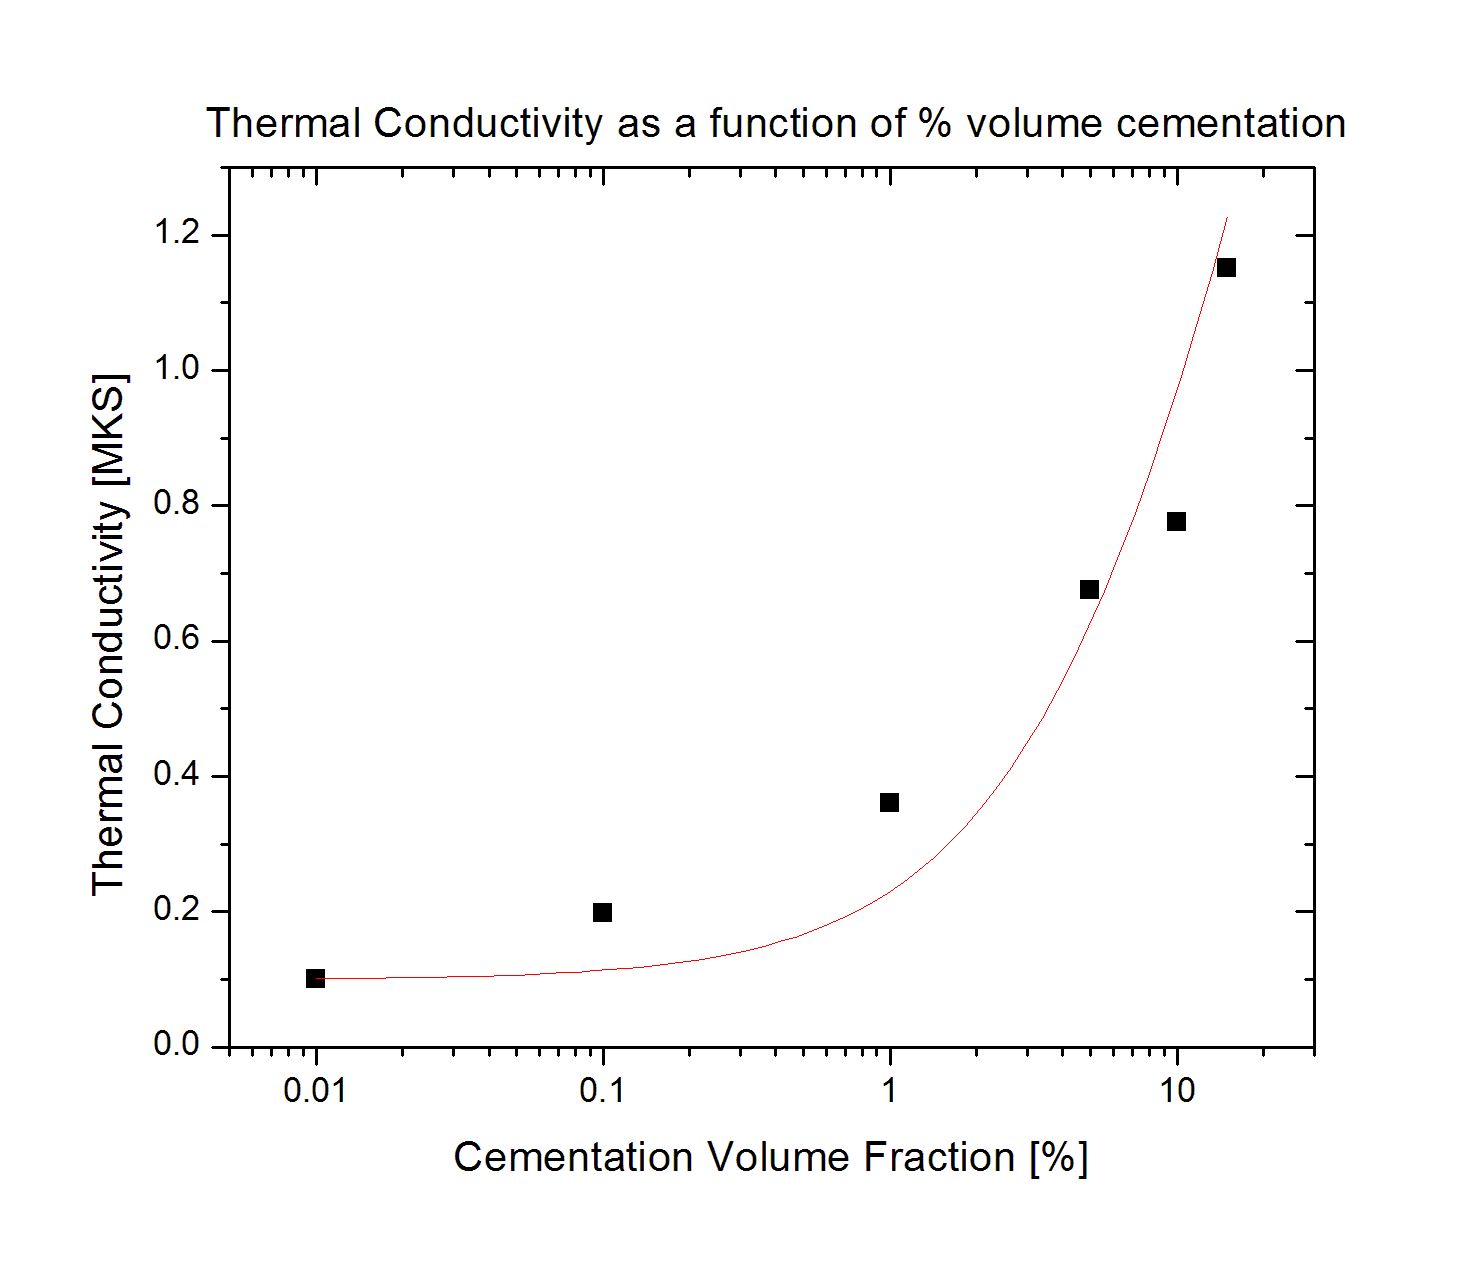
\includegraphics[width=0.57\textwidth]{PandQ2009b_CemVolumeFraction.png} }}
		\subfloat{{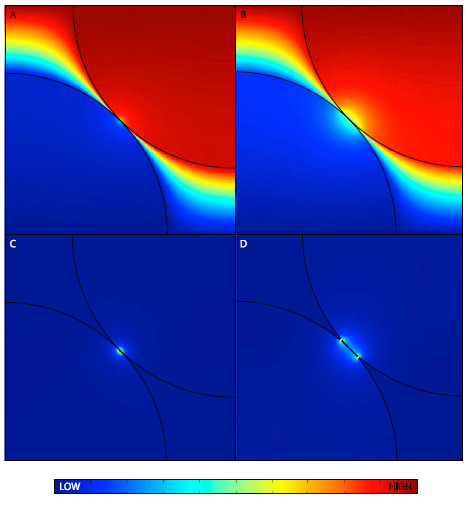
\includegraphics[width=0.43\textwidth]{PandQ2009b_Temp_grainimage.png} }}
		\caption{(Left) Thermal conductivity as a function of \% volume cementation for a 33\% porous grainy regolith. The red line represents a logarithmic fit to the data (add equation to image).  (Right) Relative temperature (a and b) and heat flux (b and c)  in a cubic centered cell from finite element numerical modeling results. Panels a and c are for a cell without bonding, and b and d represent a 0.01\% by volume pendular ring connecting the grains. The thermal conductivity of the cementation and grain material was taken to be 6 MKS and 0.937 MKS and for the interstitial gas it was 0.003 MKS in both cases. Data taken from Piqueux and Christensen (2009).}\label{fig:PCresults}
	\end{figure}

	Figure \ref{fig:PCresults}.1 shows that the thermal conductivity of the anomalous region on Mimas ($k_{eff, in} = 0.0113$ MKS) falls well below the minimum cement volume fraction considered in the modeling. The relationship between the cement volume fraction and thermal conductivity can be approximated by $k_{eff} \varpropto ln\left(1.105 (\pm 0.177)+ (VF)_{cem}\cdot 0.154 (\pm 0.177) \right)$, and it can be seen that, for vanishing gas conductivity, the volume fraction of cement ($VF_{cem}$) inside the anomaly should be $<1\times10^{-6} \%$. In fig.\ref{fig:PCresults}.2d shows that the heat flux with 0.01\% volume cementation is concentrated toward the edges of the cemented area, while for no cementation (fig.\ref{fig:PCresults}.2b) the heat flux is concentrated at the point of contact. 
	
	Important differences between these simulations and the regolith of Mimas and Tethys are that the packing structures investigated were all cubic regular packings and the grain thermal conductivity used was 0.937 MKS, much lower than for water ice and typical of basaltic glasses. However, the cement thermal conductivity used was 6 MKS, typical of crystalline ice, and since heat transfer of cemented grains is dominated by the cementation material the lower thermal conductivity of the grain should not be cause significant affect the thermal conductivity of the grain boundary region. *Grain thermal conductivity may play a more important role in determining the thermal inertia of an icy regolith due to the time scales involved.* It was shown that for very low cement volume fractions the cement thermal conductivity is negligible and the effective thermal conductivity, for the ranges of \% volume cementation evaluated, approaches a single value dependent on grain size and pore gas pressure. Though the effect of varying the grain thermal conductivity was not discussed in the paper, it can be assumed to be negligible given that heat transfer between grains is limited by the point of contact. Since the small cementation volume fractions of the order estimated by extrapolation to the low thermal conductivies of Mimas and Tethys were not considered, this model may not be sufficient to explain the small boundary conduction changes due to electron heating of grains.

\subsubsection{Maxwellian effective conductivity}
	 Wood (2011, 2013) developed a heat transfer model for grainy porous regolith based on the Maxwell equation for effective conductivity of an isotropic, heterogeneuos media. Although originally developed for electrical conductivity, the equation applies equally to thermal conductivity where the thermal paths - solid state conduction, convection through gas filled pores, and radiation from grain surfaces across pores - can be taken as acting in parallel as in Eq.\ref{eq:TCbasic}. The conductive term takes into account both solid and gas phase heat transfer and is limited depending on which phase forms a continuous path throughout the material, the lower limit corresponding to a continuous gas phase and the upper limit to a continuous solid phase. Since the lower limit is strictly valid only when the solid particles are not in contact, a non-physical situation for a regolith material, the degree of solid phase continuity is taken into account by introducing a multiplicative factor. Taking the radiative term to be negligible as discussed above, the effective thermal conductivity is given as
	
	\begin{equation}
	k_{eff} = k_{cond,min} +f_{sc}(k_{cond,max}-k_{cond,min}).
	\end{equation}
	
	For the low pressure environments of Mimas and Tethys the lower thermal conductivity limit can be taken to be zero. The upper limit depends on the thermal conductivity of the grain material $ k_{g}$, the porosity $\phi$, the volume percent and thermal conductivity of cementation region, $\chi$ and $k_{cem}$ respectively, and the fractional continuity of the solid phase $f_{sc}$. Assuming that the cementation and bulk grains are both crystalline ice ($k_{g} = k_{cem} = k_{ice}$) and that the volume percent cementation is much less than the grains ($\chi << 1-\phi$), the effective thermal conductivity becomes:	
	
	\begin{equation}
	k_{eff}=2 f_{sc} k_{ice} \frac{1-\phi}{2+\phi}
	\end{equation}
	
	The $f_{sc}$ factor represents the effect of interparticle contact and/or cementation and is a measure of the efficiency of contact between adjacent grains. The factor contains both geometrical and contact area considerations and, for uncemented soils, is given in terms of the size and number of contacts per particle, where contact size is determined by Hertzian analysis and cohesive surface forces (JKR theory).
	
	\begin{equation}
	f_{sc} = Y_{sc}N_{c} \left( \frac{N_{c}}{2\sqrt{N_{c}-1}} \frac{R_{con}}{r_{g}} \right)^{Z_{sc}}
	\end{equation}
	
	where R$_{con}$ is the radius of the contact area, r$_{g}$ is the grain radius, N$_{c}$ is the coordination number, Y$_{sc}$ is a factor determined by fitting to experimental data, and Z$_{sc}$ determines how the heat flux varies with contact radius between particles. Batchelor and O'Brien (1977) showed that the length scale for significant surface and bulk temperature variations is 
	
	$\lambda_{\nabla T} \approx \frac{r_{g}}{\alpha_{k}}$ 
	
	where 
	
	$\alpha_{k}=\frac{k_{cond}}{k_{conv}+k_{rad}}$
	
	When $R_{con} >> \lambda_{\nabla T}$, most of the heat flux is concentrated on the perimeter of the contact area and the effective thermal conductivity depends only linearly on the contact radius ($\Rightarrow Z_{sc} = 1$, see Fig.\ref{fig:PCresults}). However, when $R_{con}<\lambda_{\nabla T}$ the heat flux density is constant across the contact area and the total heat flux increases as the square of the contact radius ($\Rightarrow Z_{sc} = 2$). For the case considered here, the gas and radiative thermal conductivities are quite small meaning that $\alpha_{k}$ is large and $Z_{sc} = 1$. This differs from other thermal conductivity models considered below where the thermal conductivity is assumed to depend on the square of the contact radius. 
	
	 The coordination number can be calculated exactly for regular packings of monodisperse spheres, with N$_{c}$ = 6 for simple cubic packing which has a porosity of 47.64\%, similar to the porosity used here. For polydispersed mixtures of randomly packed particles the coordination number cannot be known exactly, but for small, cohesive, nearly spherical particles Yang et al (2000) gave a functional relationship between coordination number and porosity which closely matches measured and modeled random packings, especially at porosities $\ge40\%$. 
	
	\begin{equation}
	N_{c} = 2.02 \left( \frac{1+87.38(1-\phi)^{4}}{1+25.81(1-\phi)^{4}} \right)
	\end{equation}
	
	Using a porosity of 50\%, we find the coordination number is N$_{c}$ = 4.99. We note that for non-spherical particles the shape, orientation, and roughness of a particle can have an effect on the number of contacts and thus the porosity is less strongly coupled to the coordination number. The equilibrium contact radius between two elastic spheres of the same radius R$_{s}$ under a mechanical load can be calculated from JKR theory (Johnson et al., 1991) and is discussed in more detail for non-spherical particles by Wood (2013). An averaged best fit value of Y$_{sc}$ = 0.09 with a mean standard deviation of 13.6\% was found by fitting thermal conductivity data a variety of glass bead samples of various size distributions. Using these values and assuming a mean particle size of 50$\mu$m, we can determine the solid continuity factor, the effective contact radius, and the relative difference in contact inside and outside the anomalous regions. These values are given in Table\ref{tab:Wood2013}. 
	
	\begin{table}[c] \label{tab:Wood2013}
	\caption{Effective grain contact radius and ratio between inside and outside the anomalous regions as calculated using the theory of Wood 2013. Fitting parameters were taken from Wood (2013) and the values used for $k_{ice}$, $r_{g}$, $\phi$ and $k_{eff}$ are given in the text.}
	\centering
		\begin{tabular}{ | c | r | r | r | r | }
		 & \multicolumn{2}{| c | }{Mimas} & \multicolumn{2}{ | c |}{Tethys} \\ \hline
		 & $Z_{sc} = 1$ & $Z_{sc} = 2$ & $Z_{sc} = 1$ & $Z_{sc} = 2$ \\ \hline
		$R_{con,in}$ & $0.360 \mu m$ & $14.4 \mu m$ & 0.0519 & 0.0021 \\ \hline
		$R_{con,out}$ & $0.021 \mu m$ & $0.854 \mu m$ & 2.077 & 0.083 \\ \hline
		Ratio $\frac{R_{con,in}}{R_{con,out}}$ & 17.14 & 16.86 & 24.95 & 25.02 \\ \hline
		\end{tabular}
	\end{table}
	
	% the analysis of Wood (2013) considers thermal conductivity dependence relation to grain size where $k_{eff} \varpropto (r_{g})^{-1/3}$
	
	Taking the ratio of the contact radius values obtained from the Wood analysis, we find $\frac{R_{cont,in}}{R_{cont,out}} = 16.9$ for Mimas, while for Tethys we find $\frac{R_{cont,in}}{R_{cont,out}} = 25.0$. Interestingly, if we take the square root of these values, we find they match closely with the values obtained below.
	
\subsubsection{Analytical solutions of the heat transfer equation}

	Solutions of the heat transfer equation for spherical geometry are complicated by radiation-conduction coupling and complex packing geometries. Chan and Tien (1973) solved the equations analytically and derived explicit functional relationships between the thermal conductance of regularly packed spheres under vacuum and fundamental system parameters. This approach was adopted to describe thermal conductivity of granular regoliths and compared the theoretical results with experimental data [Gundlach and Blum, 2012]. The effective thermal conductivity was given as a function of the thermal conductivity of the solid grains, the contact radius between particles, and the packing arrangement of particles in the bulk.
	
	\begin{equation}
	k_{eff}(r_{g}, T, \phi) = k_{ice}\cdot R_{con} \cdot \xi(r_{g}, \phi)= k_{ice}(T) H(r_{g},T, \phi)
	\end{equation}

	where H is the 'Hertz-factor' used to take into account the reduction of the thermal conductivity in granular materials. The packing structure of the material and the number of intergrain contacts is taken into account by

	\begin{equation}
	\xi(r_{g}, \phi) = \frac{1}{0.531 S(\phi)} \frac{N_{A}(r_{g})}{N_{L}(r_{g})}
	\end{equation}

	Here, $S(\phi)$ is a 'model parameter' that depends on the packing structure, and $N_{A} \varpropto (r_{g})^{-2}$ and $N_{L} \varpropto (r_{g})^{-1}$ are the number of particles per unit area and unit length respectively [Chan and Tien, 1973]. If the contact radius is described by applying JKR theory, then taking the Hertz-factor as defined by the ratio of the effective and bulk thermal conductivities allows the dependence on the grain size to be determined. Futhermore, assuming a SC packing arrangement and the JKR contact radius calculated above, the expected thermal conductivity of the regolith can be calculated. In this case, calculating the ratio of the contact radius inside and outside the anomalous region is as simple as calculating the ratio of the effective thermal conductivities.It should be noted that the constants used were for regular packing arrangements and while regoliths would be expected to have random packing.
	
	\begin{align*}
	\frac{k_{eff,in}}{k_{eff,out}} \varpropto \left( \frac{r_{g,out}}{r_{g,in}} \right)
	\end{align*}
	
	\begin{table}[h] \label{tab:GBresults}
	\caption{Calculations of grain size dependence, expected regolith thermal conductivity, and contact area assuming JKR adhesion force and Hertzian contact radius. The contact radius difference was calculated assuming regolith packing was the same inside and outside the anomaly, and the estimated thermal conductivity was calculated assuming 50$\mu$ m grains, SC packing and $R_{con,JKR}$.}
		\centering
		\begin{tabular}[c]{| c | c | c | c | c | c | c | }
		& $\chi(r_{g}, \phi)$ & $\frac{r_{g,in}}{r_{g,out}}$ & \multicolumn{2}{c |}{Contact Area $(S [\mu m^{2}])$} & Ratio & $k_{eff}$ \\
		& $\frac{1}{0.531S(\phi)}\frac{N_{A}}{N_{L}}$ & $\varpropto r_{g}^{-1}$ & $\left(R_{con,JKR}\right)$ & $\left( R_{con,in}(\chi)\right)$ & $R_{con,in}/R_{con,out}$ & [MKS] \\ \hline 
		Mimas & \multirow{2}{*}{$1.88\times 10^{-2}$} & 0.59 & \multirow{2}{*}{$23.4$} & $7.37\times10^{-3}$ & 16.9 & \multirow{2}{*}{$0.637$} \\ \hline
		Tethys & & 0.40 &  & $1.53\times10^{-4}$ & 25.0 & \\ \hline
		\end{tabular}
	\end{table}
	
\subsection{Equivalent conductance modeling}

	Another method of determining the effective thermal conductivity of a porous regolith is to consider a unit cell representative of the entire particle bed and and postulating parallel heat flux through the entire cell [Zehner, 1972; Bauer, 1976; Bauer and Schl\"{u}nder, 1978; Tsostas and Martin, 1987; Steiner and K\"{o}mle, 1991]. Although this is a simplification of realistic beds, it allows for inclusion of detailed parameters representing radiation and gas thermal conductivity, particle flattening, shape, and size distribution without sacrificing ease of calculation. Taking equations presented in Tsostas and Martin (1987) and, assuming low pressure (high Knudsen numbers), the effective thermal conductivity can be written

	\begin{equation}
	k_{eff} = \left(1-\sqrt{1-\phi} \right)\phi \cdot k_{void} + \sqrt{1-\phi}\left[ H k_{ice}+(1 - H)\frac{B+1}{B}\frac{k_{ice}k_{void}}{k_{ice}+k_{void}} \right]
	\end{equation}
	
	where$k_{void}$ is the thermal conductivity across the void region due to a combination of radiative heat transfer and the latent heat of sublimation, $k_{ice}$ is the thermal conductivity of bulk ice, and $H$ is the 'Hertz-factor' used to describe particle flattening at the point of contact. The deformation factor $B$ describes the shape of the solid particle portion of the unit cell and can be related to porosity by:
	
	\begin{equation}
	B = 1.25 ( \frac{1-\phi}{\phi} )^{10/9}
	\end{equation}
	
%	Note that for a porosity of $\phi = 0.5$, the deformation factor $B = 1.25$. Using the greater value of $k_{void} = 6.3\times10^{-6} \frac{J}{m \cdot s \cdot K}$ from the analysis above and a thermal conductivity for ice at 80 K of $k_{ice} = 567/T = 7.09 \frac{J}{m \cdot s \cdot K}$, we can analyze the effective thermal conductivity to obtain a comparison of the Hertz factor inside and outside the thermal anomally feature.

	Taking the thermal conductivity of the void region to be negligible as discussed above, we can simplify the effective thermal conductivity to depend only on the Hertz factor and the porosity of the regolith.
	
	\begin{equation}\label{eq:unitcell}
	\Rightarrow k_{eff} \approx \sqrt{1-\phi}\cdot H \cdot k_{ice}(T)
	\end{equation}
	
	 Using the effective thermal conductivities obtained above for a 50\% porous regolith both inside and outside the anomalies and taking the thermal conductivity of water ice at 80Kto be $k_{ice} = 567/T = 7.09$ MKS [Kossacki et al., (1994)], we can solve for the Hertz-factor (Table 1). In this instance, the Hertz-factor was taken as an empirical parameter that was determined by fitting to experimental data, and values obtained previously to describe sand particles [Tsostas and Martin, 1987] and a porous icy cometary nucleus [Steiner and K\"{o}mle, 1991] are on the order of  $H  \approx (1 - 4) \times10^{-3}$ [SteinerKomle1991] compare favorably with the values obtained for the icy regoliths considered here. Kossacki et al. (1994), using the same analysis, assumed that the Hertz-factor was related to the square of the particle contact radius so that
	
	\begin{equation}
	\Rightarrow \frac{R_{con,in}}{R_{con,out}} = (\frac{H_{n, in}}{H_{n, out}})^{1/2} \varpropto \left( \frac{k_{eff,in}}{k_{eff,out}} \right)^{1/2}
	\end{equation}
	
	from which we find that $\frac{R_{con,in}}{R_{con,out}} = 4.17$ Mimas and $5$ for Tethys, meaning the effective radius of contact is greater inside the anomalies than outside and of the same order for the two bodies.
	
\subsection{Effective Medium Theory approach}

	Thermal conductivity in porous granular regoliths has several similarities to percolation of electricity through mixed media of differing conductivities, and similar mathematical approaches can be used to study both. Below a certain volume percentage of conductive material the effective conductivity of the mixture is effectively zero, while once a certain critical concentration is reached the conductivity increases sharply and continues to increase with increasing volume percent of conductive material. The material can be viewed as an effective-medium to estimate the effective thermal conductivity for a random network of spherical grains arranged on a regular lattice  [Sirono and Yamamoto, 1997; Kirkpatrick, 1973]. Integrating the probability distribution of $k$ multiplied by the 1-D heat flux to obtain the effective heat flux and taking the thermal conductivity of the void space to be zero, the effective thermal conductivity is given by
	
%	\begin{equation}
%	\frac{k_{eff} - k_{ice}}{k_{ice} +(1/p_{c}-1)k_{eff}}p + \frac{k_{eff}-k_{void}}{k_{void}+(1/p_{c}-1)k_{eff}}(1-p)=0
%	\end{equation}
	\begin{equation}
	k_{eff} = k_{ice} \frac{p - p_{c}}{1 - p_{c}}
	\end{equation}

	where the probability of a lattice site being occupied or packing fraction is $p$ and $p_{c}$ is the percolation threshold which defines the minimum packing fraction for a continuous thermal path to exist across the material. However, this expression does not consider the limitation of heat flow due to reduced area at the grain contacts. This effect can be taken into account by multiplying by a factor dependent on packing structure, grain size and effective contact radius similar to that found by Hertzian analysis.
	 
	\begin{equation}
	k_{eff} = k_{ice} ( \frac{p - p_{c}}{1-p_{c}} )\frac{\pi R_{con}^{2}}{g r_{g}^{2}}
	\end{equation}

	where $g$ is a geometrical factor dependent on the packing structure and $g = 4$ for a cubic lattice. Assuming a simple cubic packing structure of the grains, the relation between porosity and the packing fraction is
	
	\begin{equation}
	p = \left[ \frac{4 \pi}{3} \left( \frac{1}{2} \right)^{3} \right]^{-1} (1 - \phi) \\
	\end{equation}
	
	and the critical packing fraction $p_{c} = 1/3$. The contact radii calculated using this method are given in table 1, and the ratio of the contact radius inside and outside the anomaly is $\frac{R_{con,in}}{R_{con,out}} = ( \frac{S_{in}}{S_{out}} )^{1/2} = 4.14$ for Mimas and $5.0$ for Tethys. This is in very close argreement with the value obtained from the analysis of Kossacki et al.
	% Sirono and Yamamoto use $k_{eff} \varpropto (r_{g})^{-2/3}$. The results from these calculations are presented in table \ref{tab:HertzGrain}.

	\begin{table}
		\hspace{-1.5 cm}{
		\begin{tabular}[ h, font=small ]{ l | l | c | c | c | c | c }
	\multicolumn{2}{c | }{Authors} & Howett (2011, 2012) & \multicolumn{2}{ | c |}{Wood (2013)} & S\&K (1991) & S\&Y (1997) \\ \hline
	& Location & $k_{eff} \left[ \frac{J}{m\cdot s\cdot K} \right]$ & $f_{sc}$ & $R_{con} [\mu m]$ & H [cm$^{-1/3}$] & S [$\mu m^{2}$]\\  \hline
	Mimas & Inside anomaly & $1.13 \times 10^{-2}$ & $3.98 \times 10^{-3}$ & 0.354 & $2.25 \times10^{-3}$ & 17.1 \\
		& Outside anomaly & $< 6.7 \times 10^{-4}$ &  $2.36 \times 10^{-4}$ & .021 & $1.3 \times10^{-4}$ & 1.00 \\ \hline
	Tethys & Inside anomaly & $1.63 \times 10^{-3}$ &  $5.75 \times 10^{-4}$ & 0.051 & 3.25 $\times10^{-4}$ & 2.47 \\
		& Anomaly boundary &  $3.16 \times 10^{-4}$ &  $1.11 \times 10^{-4}$ & 0.028 & 6.30 $\times10^{-5}$ & 0.48 \\
		& Outside anomaly & $6.53 \times 10^{-5}$ &  $2.30 \times 10^{-5}$ & 0.006 & 1.30 $\times10^{-5}$ & 0.01 \\
	\end{tabular} }
	\caption{Contact radii calculated using the various thermal conductivity theories presented above. For all analyses, we see that the contact area inside the anomalous region is greater than without, which is in agreement with the increased thermal conductivity for all other factors being constant.}
	\end{table}
	
\end{document}